%%%%%%%%%%%%%%%%%%%%%%%%%%%%%%%%%% NAME %%%%%%%%%%%%%%%%%%%%%%%%%%%%%
%%%%%%%%%%%%%%%%%
\section{Introduction}

\begin{frame}{Introduction}{Overview}
  \begin{figure}[H]
	\centering
	%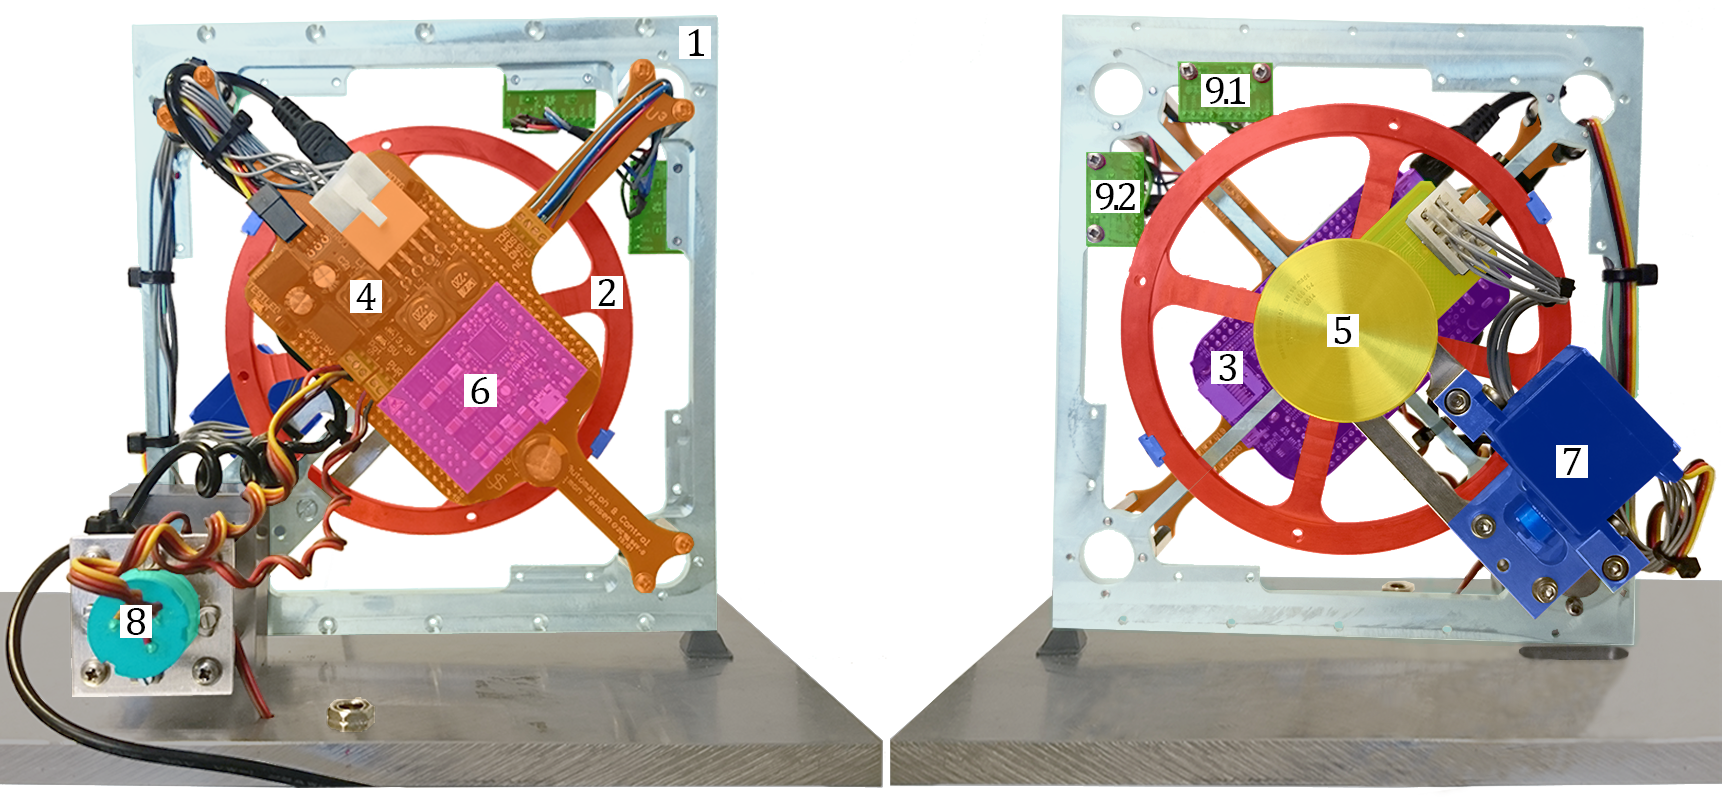
\includegraphics[scale=0.65]{Pictures/Cubli12.png}
  \end{figure}
\end{frame}

% ---------------------------------------------------
\section{System Description}

\begin{frame}{System Description}{Overview}

  \begin{minipage}{\linewidth}
  	\begin{minipage}{0.45\linewidth}
  		\begin{figure}[H]
  			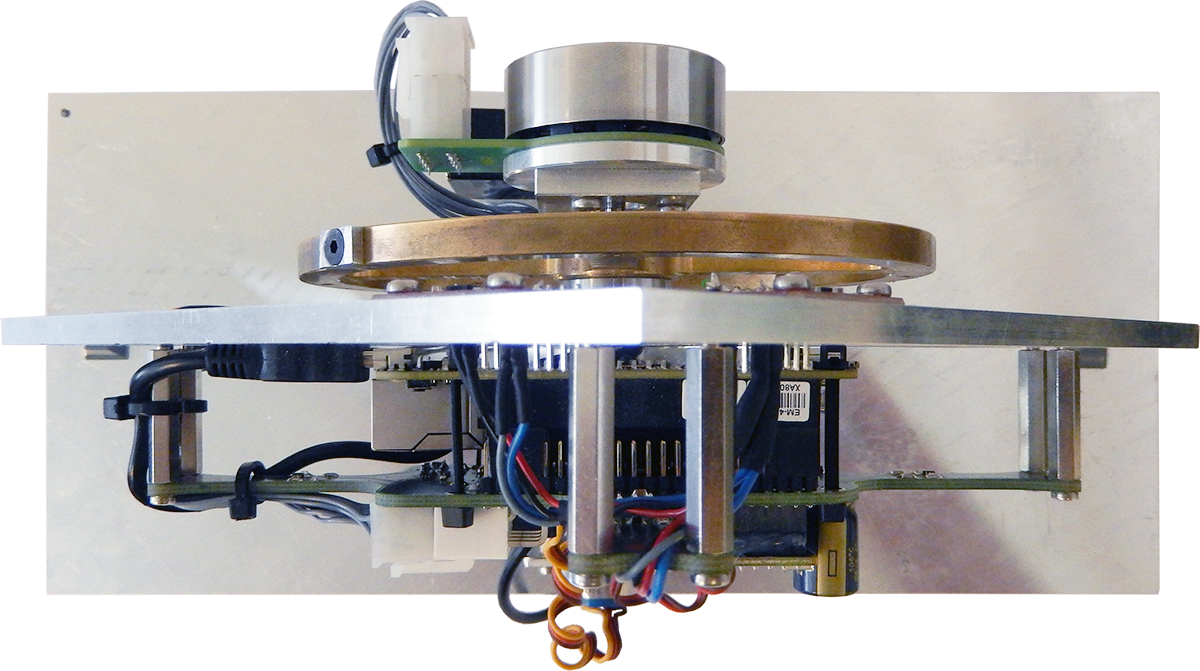
\includegraphics[scale=0.5]{Pictures/Cubli-3.png}
  			\centering
  		\end{figure}
  	\end{minipage}
  	\hspace{0.03\linewidth}
  	\begin{minipage}{0.45\linewidth}
  		\begin{figure}[H]
  			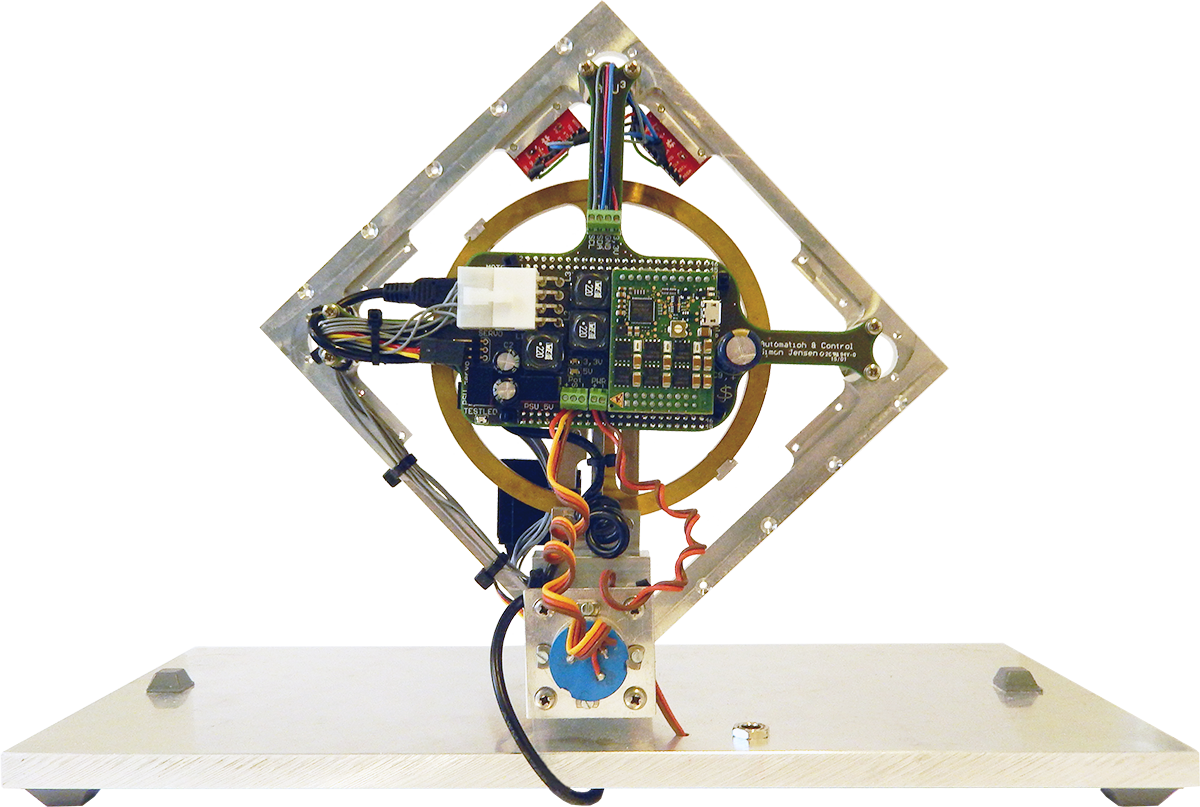
\includegraphics[scale=0.5]{Pictures/Cubli-1.png}
  			\centering
  		\end{figure}
  	\end{minipage}
  \end{minipage}

\end{frame}

\begin{frame}{System Description}{Overview}
	\begin{figure}[H]
		\centering
		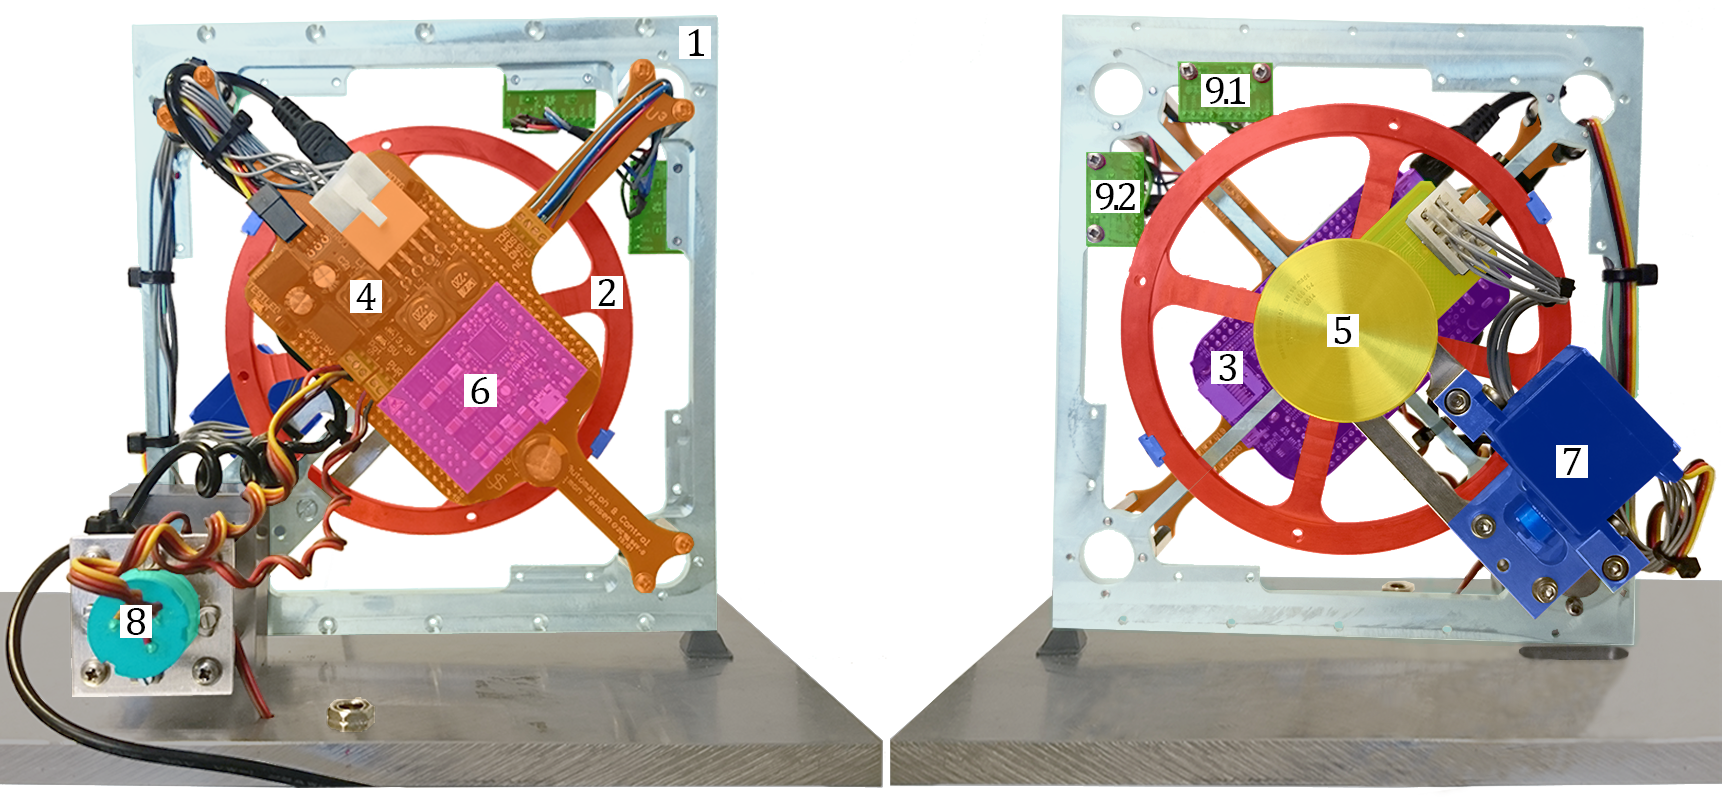
\includegraphics[scale=0.16]{Pictures/Cubli12.png}
	\end{figure}
\end{frame}

% -------------------------------------------------------
\section{Requirements}

\begin{frame}{Requirements}{Overview}
\begin{itemize}
 \item {Keep balancing from unstable equilibrium position}
  \begin{itemize}
	\item {Starting out from equilibrium position at null velocity}
	\linebreak
\end{itemize}
\item {The prototype should be able to balance around 0 rad}
	\begin{itemize}
	\item {Changing angle of baseplate within reasonable range}
	\end{itemize}
\end{itemize}


\end{frame}

% -----------------------------------------------------------------
\section{Model}

\begin{frame}{Model}{Overview}
	\begin{figure}[H]
		\centering
		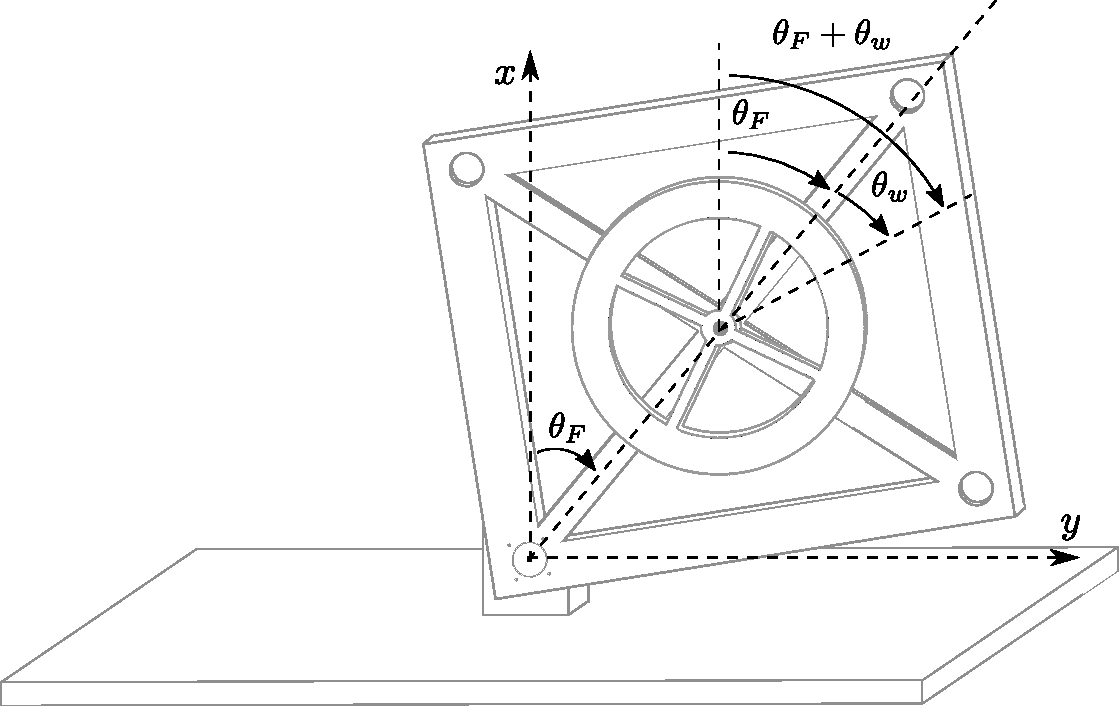
\includegraphics[scale=0.5]{Pictures/mechanicalSystem.pdf}
	\end{figure}
\end{frame}

\begin{frame}{Model}{freebody diagram of the wheel}
	\begin{figure}[H]
		\centering
		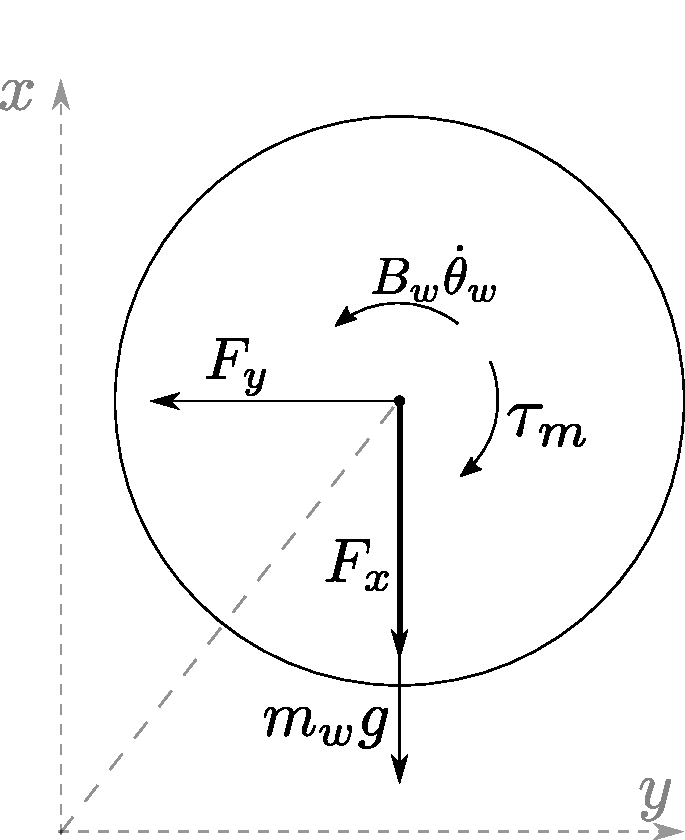
\includegraphics[scale=0.40]{Pictures/freeBodyWheel.pdf}
	\end{figure}
	\begin{displaymath}	
	  \si{ J_w (\vec{\ddot{\theta}_F} + \vec{\ddot{\theta}_w}) =} 
	  \si{ \vec{\tau_m} - B_w \vec{\dot{\theta}_w }}
	\end{displaymath}
\end{frame}

\begin{frame}{Model}{freebody diagram of the frame}
	\begin{figure}[H]
		%\centering
		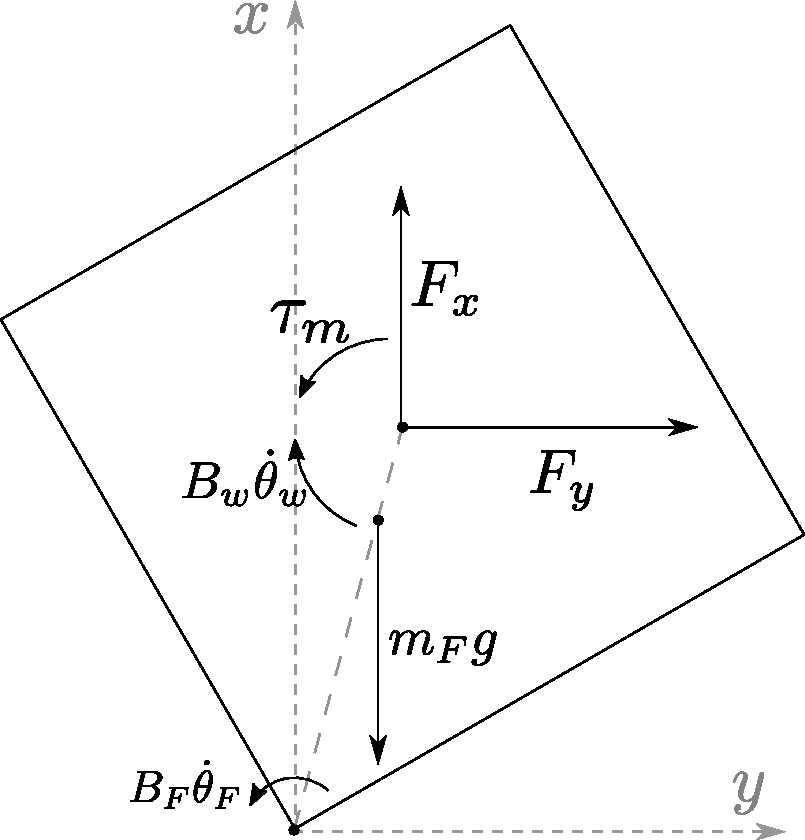
\includegraphics[scale=0.40]{Pictures/freeBodyFrame.pdf}
	\end{figure}
	\begin{displaymath}
	\si{J_F \vec{\ddot{\theta}_F} =}
	\si{-B_F \vec{\dot{\theta}_F} + \vec{l_F} \times (m_F\cdot \vec{g}) + \vec{l_w} \times \vec{F} - \vec{\tau_m} + B_w \vec{\dot{\theta}_w}}
	\end{displaymath}
	
	
\end{frame}

\begin{frame}{Model}{Construction}
	\begin{figure}[H]
		\centering
		%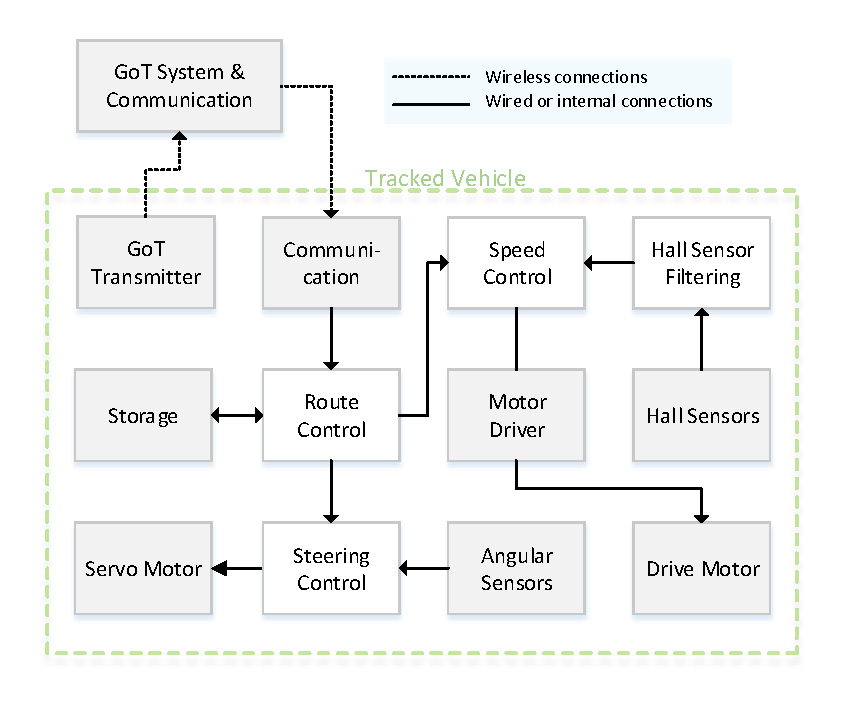
\includegraphics[scale=0.65]{Pictures/SO3.pdf}
	\end{figure}
\end{frame}

\begin{frame}{Model}{Linearization}
	\begin{figure}[H]
		\centering
		%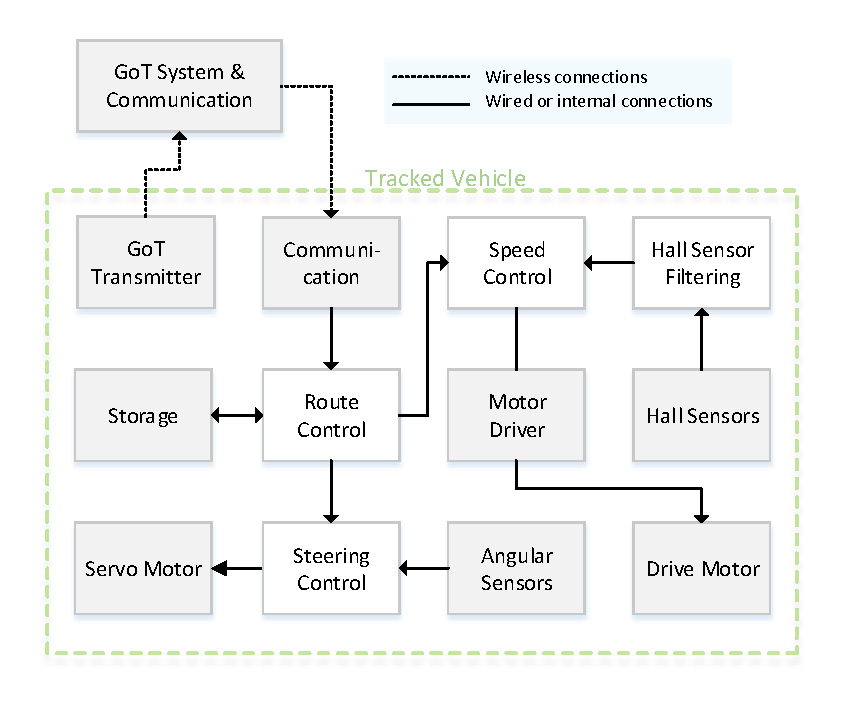
\includegraphics[scale=0.65]{Pictures/SO3.pdf}
	\end{figure}
\end{frame}

\begin{frame}{Model}{Linearization}
	\begin{figure}[H]
		%\centering
		%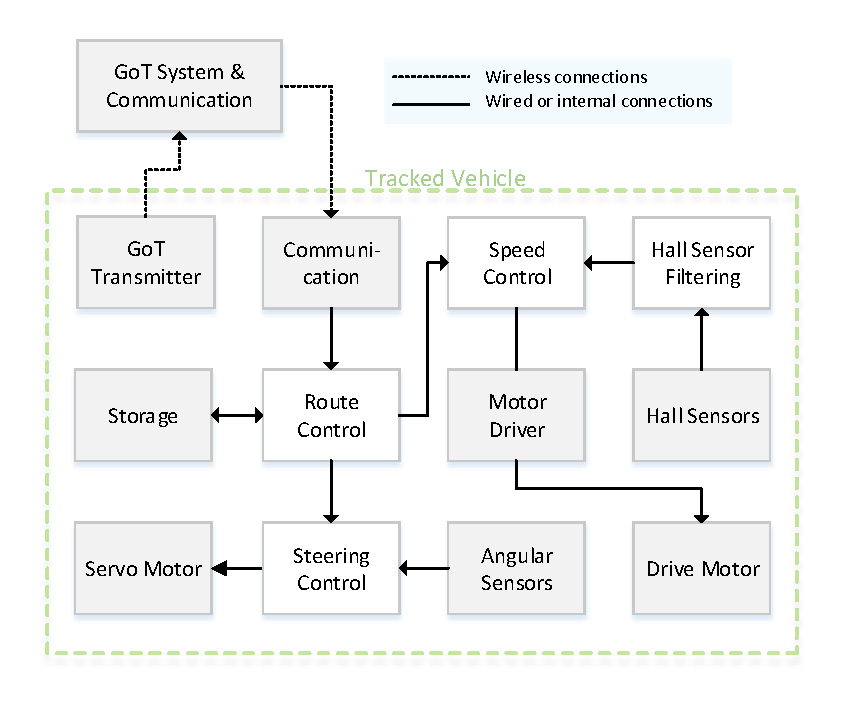
\includegraphics[scale=0.65]{Pictures/SO3.pdf}
	\end{figure}
		\begin{flalign}
		&\si{(J_F+m_w \cdot {l_w}^{2}) \Delta \ddot{\theta}_F =}& \nonumber \\
		&\si{-B_F \Delta \dot{\theta}_F +  ( m_F \cdot l_F + m_w \cdot l_w ) \cdot g \cdot \Delta \theta_F - \Delta \tau_m + B_w \Delta \dot{\theta}_w }& \nonumber
		\end{flalign}
		
\end{frame}

\begin{frame}{Model}{Blockdiagram}
	\begin{figure}[H]
		\centering
		  \begin{tikzpicture}[ auto,
                       thick,                         %<--setting line style
                       node distance=1.5cm,             %<--setting default node distance
                       scale=0.48,                     %<--|these two scale the whole thing
                       every node/.style={scale=0.58}, %<  |(always change both)
                       >/.tip={Triangle[angle=40:5pt]}
                       ]

    %-- Blocks creation --%
    \draw
      % DIRECT TERM %
      node[shape=coordinate][](input1) at (0,0){}
      node[shape=coordinate][](feedForward) at (0.5,0){}
      node(sum1) at (7.75,0) [sum] {\si{\sum}}
      node(sum2) at (9.25,0) [sum]{\si{\sum}}
      node(sum3) at (10.75,0) [sum]{\si{\sum}}

      node(torque2rotacc1) at (12.85,0) [block]{\large \si{\frac{1}{J_F + m_w \cdot {l_w}^{2}}}}

      node(integration1) at (15.75,0) [block] {\large \si{\frac{1}{s}}}
      node(integration2) at (18.2,0) [block] {\large \si{\frac{1}{s}}}

      node[shape=coordinate][](output) at (19,0){}
      node[shape=coordinate][](veloFeedbackNode) at (16.8,0){}
      node[shape=coordinate][](accFeedbackNode) at (14.5,0){}
    ;
    \draw
      % REACTION WHEEL EQUATIONS %  
      node(sum4) at (1.5,-1.6) [sum]{\si{\sum}}
      node(sum5) at (2.85,-1.6) [sum]{\si{\sum}}

      node(torque2rotacc2) at (4.3,-1.6) [block]{\large \si{\frac{1}{J_w \cdot s}}}
      % node(integration3) [block, right of = torque2rotacc2] {$\frac{1}{s}$}
      node(frictionWheel) at (6.9,-1.6) [block] {\large $B_w$}

      node[shape=coordinate][](veloWheelFeedback) at (7.75,-3.2){}
    ;
    \draw
      % FEEDBACKS %
      node(accFeedback) at (8, -4.8) [block] {\large \si{J_w}}
      node(veloFeedback) at (12.65,-1.6) [block] {\large \si{B_F}}
      node(angleFeedback) at (11.65,-3.2) [block] {\large \si{(m_F \cdot l_F + m_w \cdot l_w)g}}
    ;
    %-- Block linking --%
    % INPUT %
    \draw[-](input1)        -- node{\large \si{\tau_m(s)}}(feedForward);
    \draw[->](feedForward)  -- (sum1);

    % OUTPUT %
    \draw[-](integration2)  -- (output);
    \draw[->](output)       -- node {\large \si{\theta_{F}(s)}} (20,0);

    % DIRECT TERM %
    \draw[->] (sum1)            -- (sum2);
    \draw[->] (sum2)            -- (sum3);
    \draw[->] (sum3)            -- (torque2rotacc1);
    \draw[->] (torque2rotacc1)  -- node{\large \si{\ddot{\theta}_F(s)}}(integration1);
    \draw[->] (integration1)    -- node{\large \si{\dot{\theta}_F(s)}}(integration2);

    % REACTION WHEEL EQUATIONS %
    \draw[->] (feedForward)     |- (sum4);
    \draw[->] (sum4)            -- (sum5);
    \draw[->] (sum5)            -- (torque2rotacc2);
    \draw[->] (torque2rotacc2)  -- node{\large \si{\dot{\theta}_w(s)}}(frictionWheel);
    % \draw[->] (integration3)    -- (frictionWheel);
    \draw[->] (frictionWheel)   -| (sum1);

    \draw[-] (frictionWheel)       -| (veloWheelFeedback);
    \draw[->] (veloWheelFeedback)  -| (sum5);

    % FEEDBACKS
    \draw[->] (accFeedbackNode)  |- (accFeedback);
    \draw[->] (accFeedback)      -| (sum4);

    \draw[->] (output)           |- (angleFeedback);
    \draw[->] (angleFeedback)    -| (sum2);

    \draw[->] (veloFeedbackNode) |- (veloFeedback);
    \draw[->] (veloFeedback)     -| (sum3);

    %-- Nodes --%
    \draw%--------------------------------------------------------------
      node at (input1)            [shift={(-0.04, -0.05 )}] {\large \textbullet}
      node at (output)            [shift={( 0.007, -0.05 )}] {\large \textbullet}
      node at (veloFeedbackNode)  [shift={( 0.007, -0.05 )}] {\large \textbullet}
      node at (accFeedbackNode)   [shift={( 0.007, -0.05 )}] {\large \textbullet}
      node at (feedForward)       [shift={( 0.007, -0.05 )}] {\large \textbullet}
      node at (frictionWheel)     [shift={( 0.70, -0.04 )}] {\large \textbullet}
    ;

    %-- Summation signs --%
      \draw%--------------------------------------------------------------
      node at (sum1) [right = -6.6mm, below = .6mm] {$-$}
      node at (sum1) [right = -3mm, below = 3.9mm]  {$+$} 
      node at (sum2) [right = -6.6mm, below = .6mm] {$+$}
      node at (sum2) [right = -3mm, below = 3.9mm]  {$+$}
      node at (sum3) [right = -6.6mm, below = .6mm] {$+$}
      node at (sum3) [right = -3mm, below = 3.9mm]  {$-$}
      node at (sum4) [right = -6.6mm, below = .6mm] {$+$}
      node at (sum4) [right = -3mm, below = 3.9mm]  {$-$}
      node at (sum5) [right = -6.6mm, below = .6mm] {$+$}
      node at (sum5) [right = -3mm, below = 3.9mm]  {$-$}
    ;

  \end{tikzpicture}
	\end{figure}
\end{frame}
%\section{Hardware and Software}
%%%%%%%%%%%%%%%%%
%\subsection{Prototype overview}
%
%\begin{frame}{Hardware and Software}{Prototype overview}
%  \begin{figure}[H]
%	\centering
%	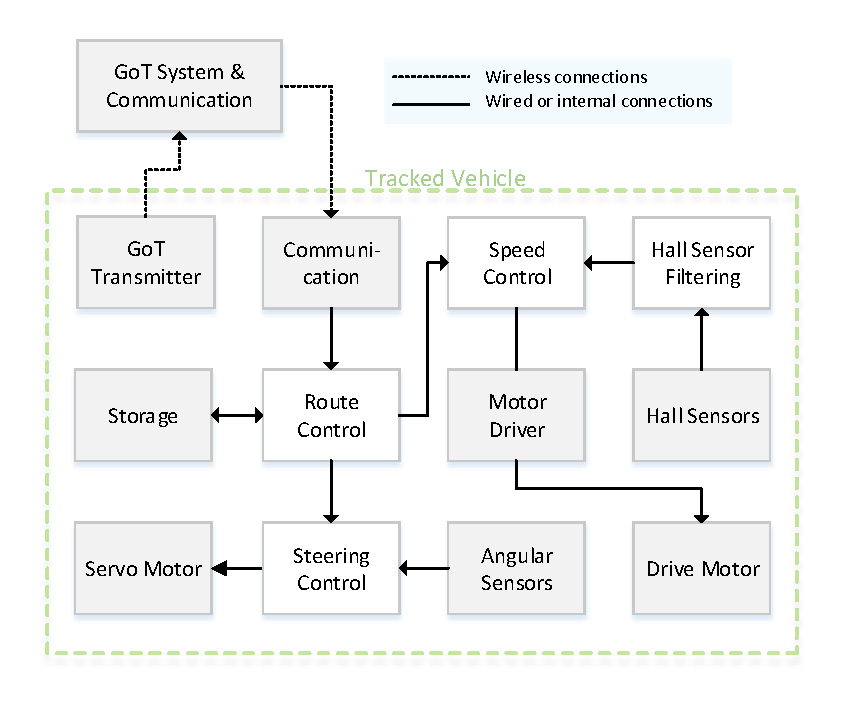
\includegraphics[scale=0.65]{Pictures/SO3.pdf}
%  \end{figure}
%\end{frame}
%%%%%%%%%%%%%%%%%
%
%%%%%%%%%%%%%%%%%
%\subsection{Hardware components}
%
%\begin{frame}{Hardware and Software}{Hardware components}
%\textbf{Controller}
%\begin{itemize}
%\item{Arduino Mega 2560}
%\end{itemize}
%  \begin{figure}[H]
%	\centering
%	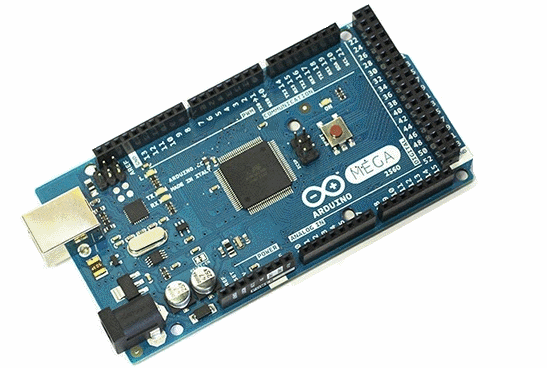
\includegraphics[scale=0.4]{Pictures/ArduinoMega.png}
%  \end{figure}
%\end{frame}
%
%\begin{frame}{Hardware and Software}{Hardware components}
%\textbf{Velocity Sensor}
%\begin{itemize}
%\item{Hall Sensor}
%\end{itemize}
%  \begin{figure}[H]
%	\centering
%	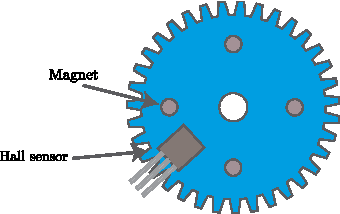
\includegraphics[scale=1.5]{Pictures/hallSensorDrawing.pdf}
%  \end{figure}
%\end{frame}
%
%\begin{frame}{Hardware and Software}{Hardware components}
%\textbf{Angular Sensor}
%\begin{itemize}
%\item{HMC5883L Magnetometer}
%\end{itemize}
%
%  \begin{minipage}{\linewidth}
%  	\begin{minipage}{0.45\linewidth}
%  		\begin{figure}[H]
%  			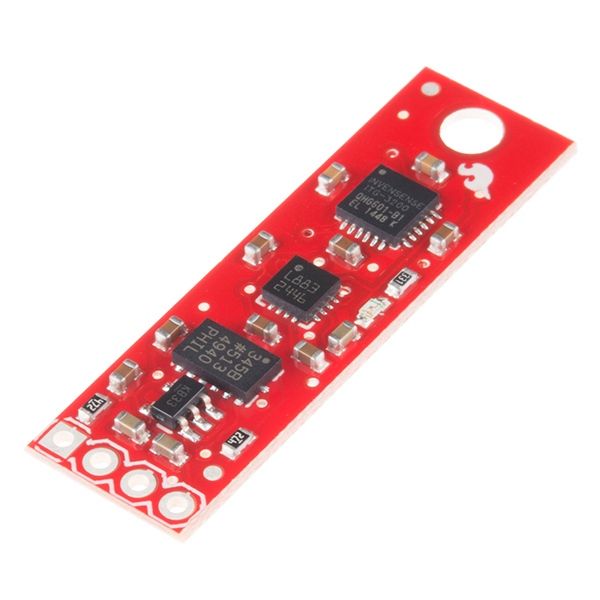
\includegraphics[scale=0.7]{Pictures/NineDegree.jpg}
%  			\centering
%  		\end{figure}
%  	\end{minipage}
%  	\hspace{0.03\linewidth}
%  	\begin{minipage}{0.45\linewidth}
%  		\begin{figure}[H]
%  			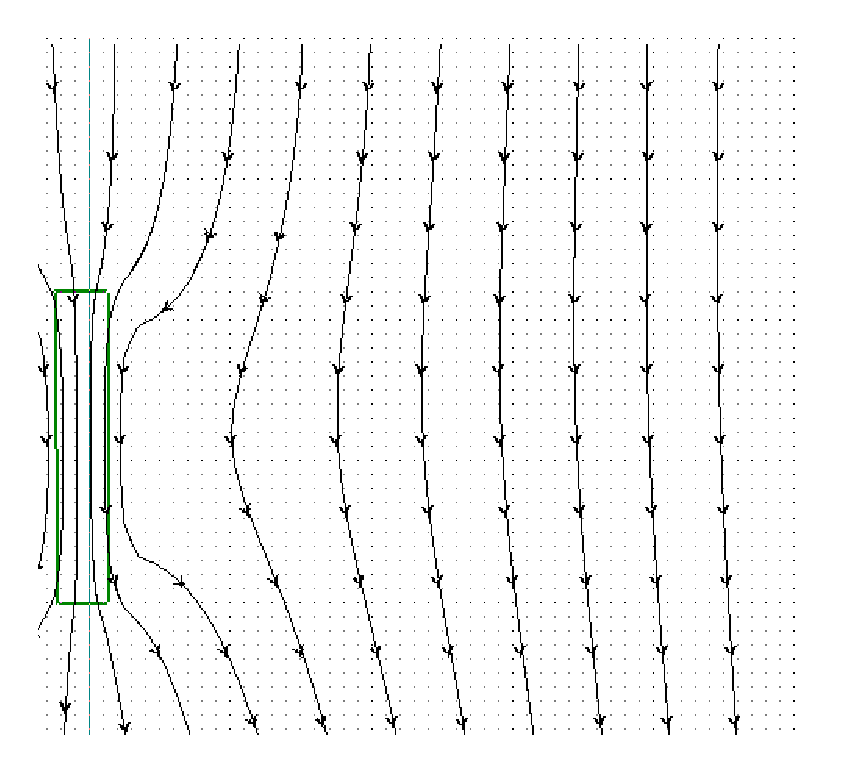
\includegraphics[scale=0.35]{Pictures/Magne.pdf}
%  			\centering
%  		\end{figure}
%  	\end{minipage}
%  \end{minipage}
%
%\end{frame}
%
%
%
%
%\begin{frame}{Hardware and Software}{Hardware components}
%\textbf{Position Sensor}
%\begin{itemize}
%\item{Games on Track system (GoT)}
%\end{itemize}
%  \begin{figure}[H]
%	\centering
%	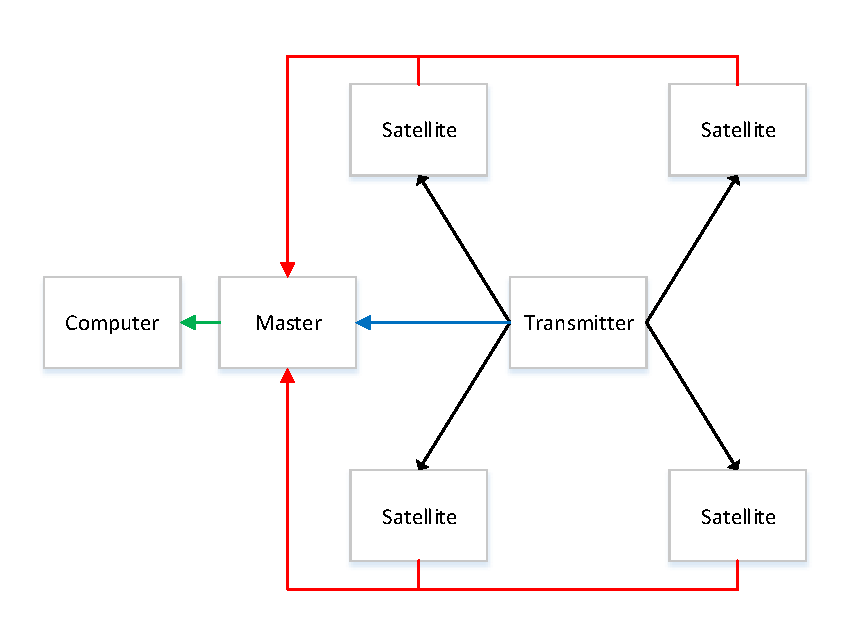
\includegraphics[scale=0.6]{Pictures/GOTNew.pdf}
%  \end{figure}
%\end{frame}
%
%\begin{frame}{Hardware and Software}{Hardware components}
%\begin{itemize}
%\item {Communication}
%\item {Storage}
%\item {Motor driver}
%\item {Battery and Power monitor}
%\end{itemize}
%\end{frame}
%%%%%%%%%%%%%%%%%
%
%%%%%%%%%%%%%%%%%
%\subsection{Software}
%
%\begin{frame}{Hardware and Software}{Software}
%\begin{itemize}
% \item {Real Time Operating System}
%  \begin{itemize}
%	\item {KRNL by Jens Dalsgaard Nielsen}
%\end{itemize}
%\end{itemize}
%
%  \begin{figure}[H]
%	\centering
%	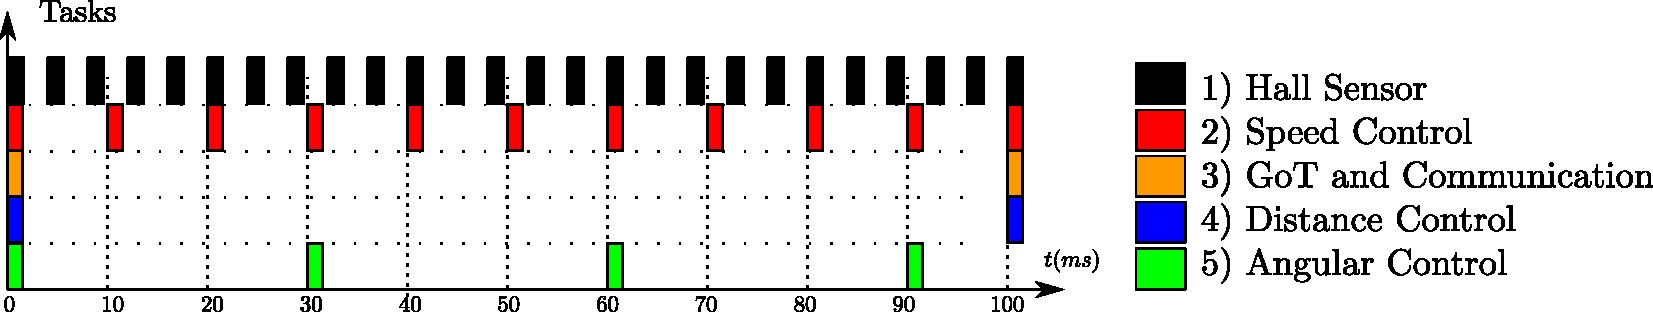
\includegraphics[scale=0.35]{Pictures/scheduleRequest.pdf}
%  \end{figure}
%
%  \begin{figure}[H]
%	\centering
%	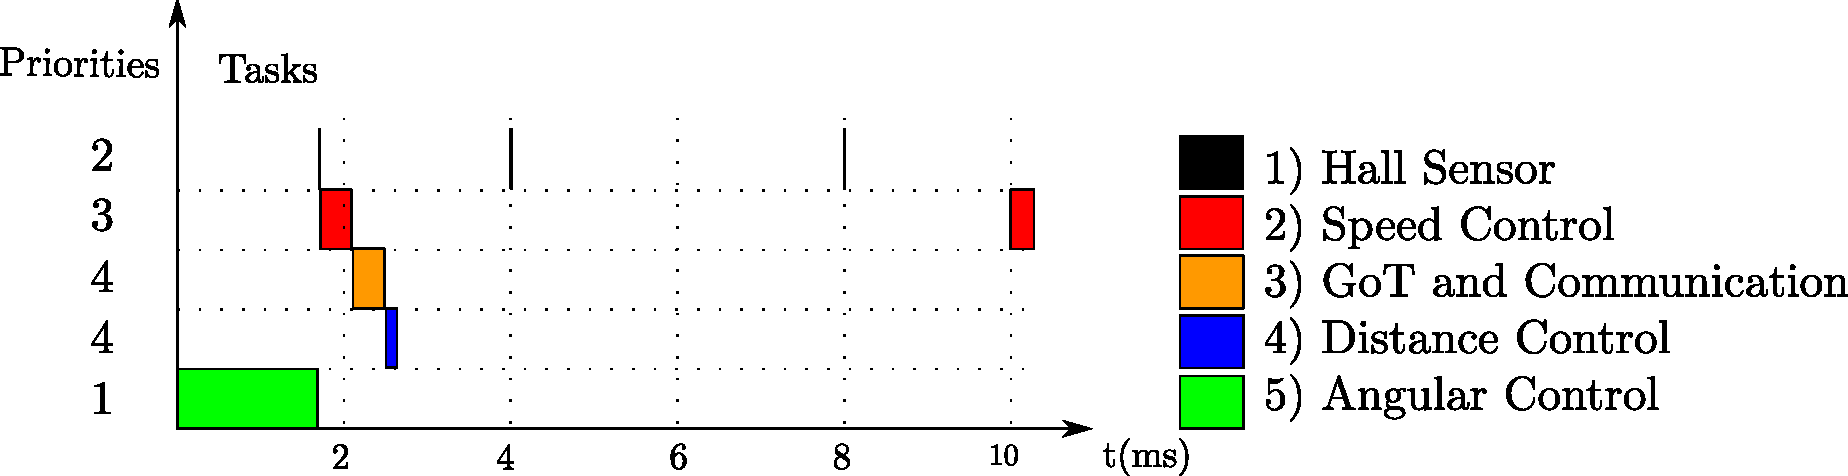
\includegraphics[scale=0.3]{Pictures/schedulePriorities.pdf}
%  \end{figure}
%\end{frame}